%!TEX root = ../main.tex

\section{Surface triangulation and subdivision}
\label{sec:surface_triangulation_subdivision}

\subsection{Surface triangulation}

Before triangulating, we need to define whether Voronoi cells belong to the same surface neighborhood or not. 
In comparison to the typical Delaunay dual-triangulation obtained from a Voronoi diagram, here we don't want to connect by an edge every pair of Voronoi cells having a common frontier in 2D. Some cells belong to different surface areas and then shouldn't be linked together.
For this we will use the borders that were constructed in \ref{sec:border_marking}.
We consider that two Voronoi cells $V_i$ and $V_j$ are belonging to the same neighborhood if there is no border separating them. In other words, we say that $V_i$ and $V_j$ are neighbors if there exists at least one non-border pixel belonging to $V_i$ which is neighbor (considering the 6-neighborhood we defined in Fig. \ref{fig:pixel_neighborhood}) to at least 1 pixel of the pixels belonging to $V_j$.

\begin{figure}[ht]
\centering
\scalebox{0.05}{
\begin{tikzpicture}[spy using outlines={circle,red,magnification=7.5,size=40cm, connect spies}]
\node {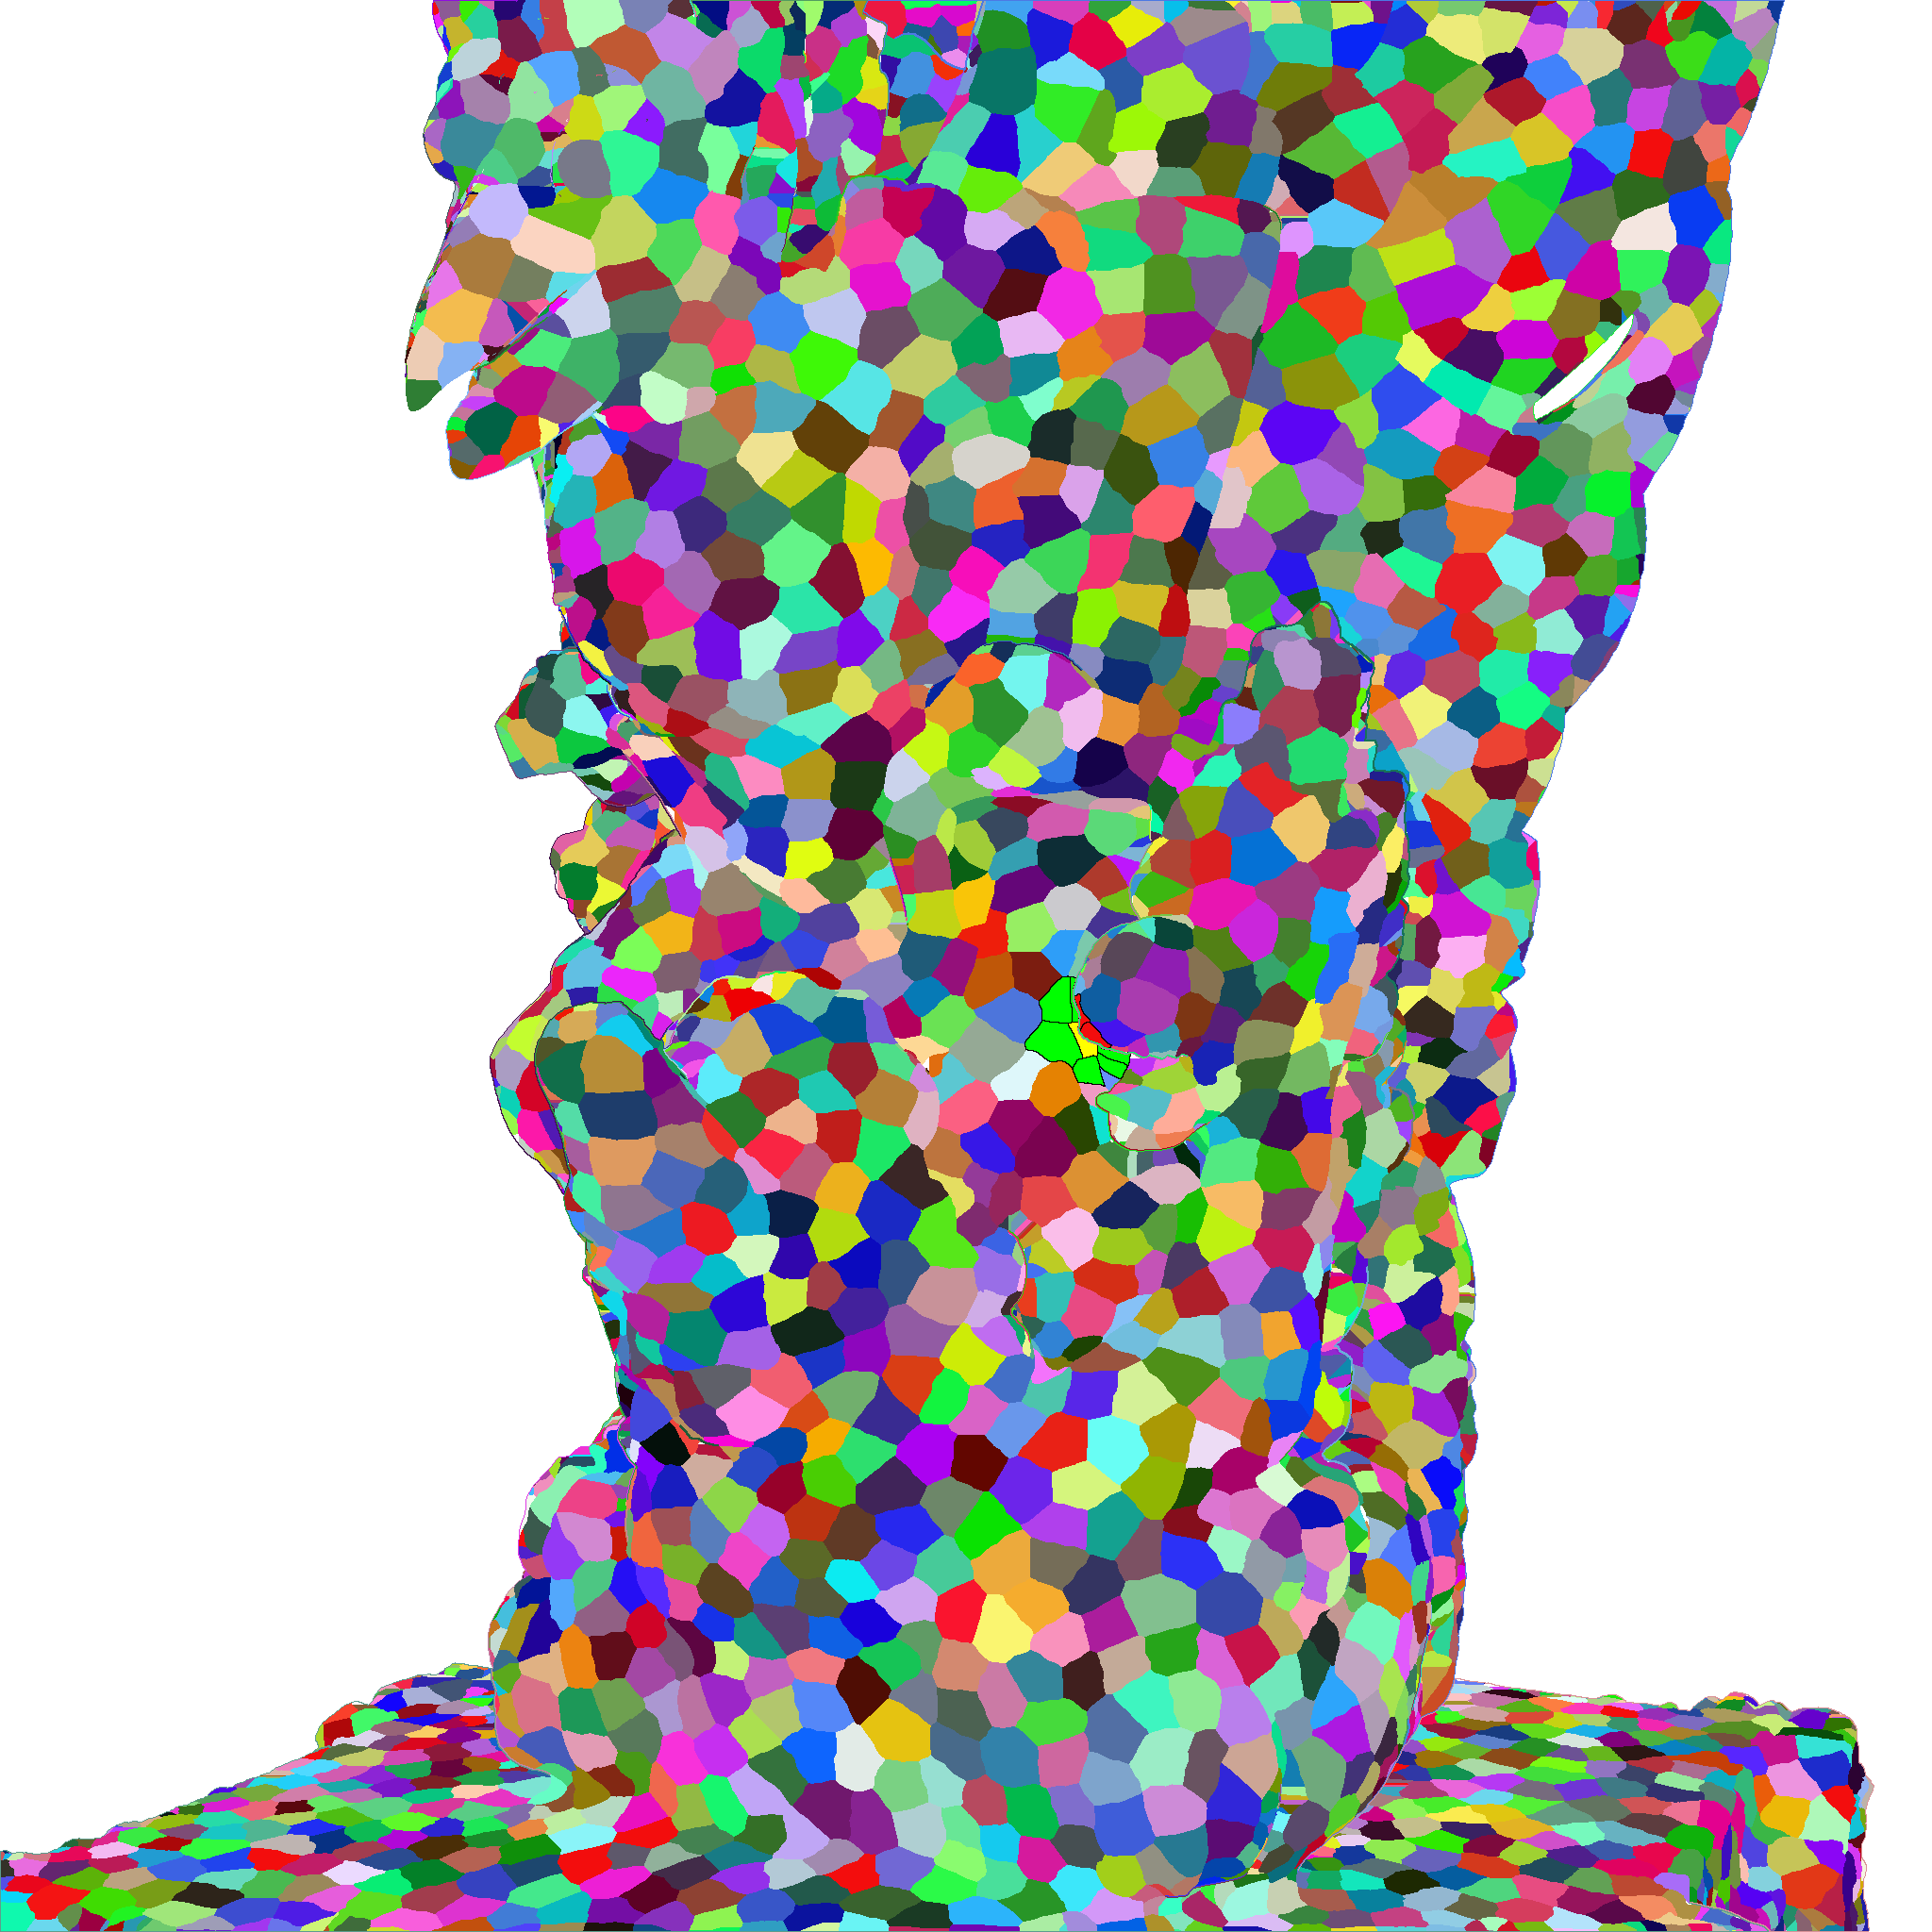
\includegraphics{Images/VoronoiDiagram3DBordersNeighborhood-Garuda}};
\spy on (4.25,-2.75) in node [left] at (100,-2.75);
\end{tikzpicture}
}
\caption{Neighborhood of a Voronoi cell (in yellow) $V$. In all the cells that have a common frontier with $V$ in 2D, the cells colored in green belong to the neighborhood of the cell on the surface, whereas the ones colored in red don't.}
\label{fig:voronoi_cell_neighborhood}
\end{figure}

Considering the neighborhoods computed, we define our triangulation as being an altered dual representation of a Voronoi diagram, where edges are only connecting cells belonging to the same neighborhood (Figure \ref{fig:voronoi_diagram_triangulation}).
This allow to generate a triangulation where only points belonging to the same surface areas are triangulated together.

\begin{figure}[ht]
\centering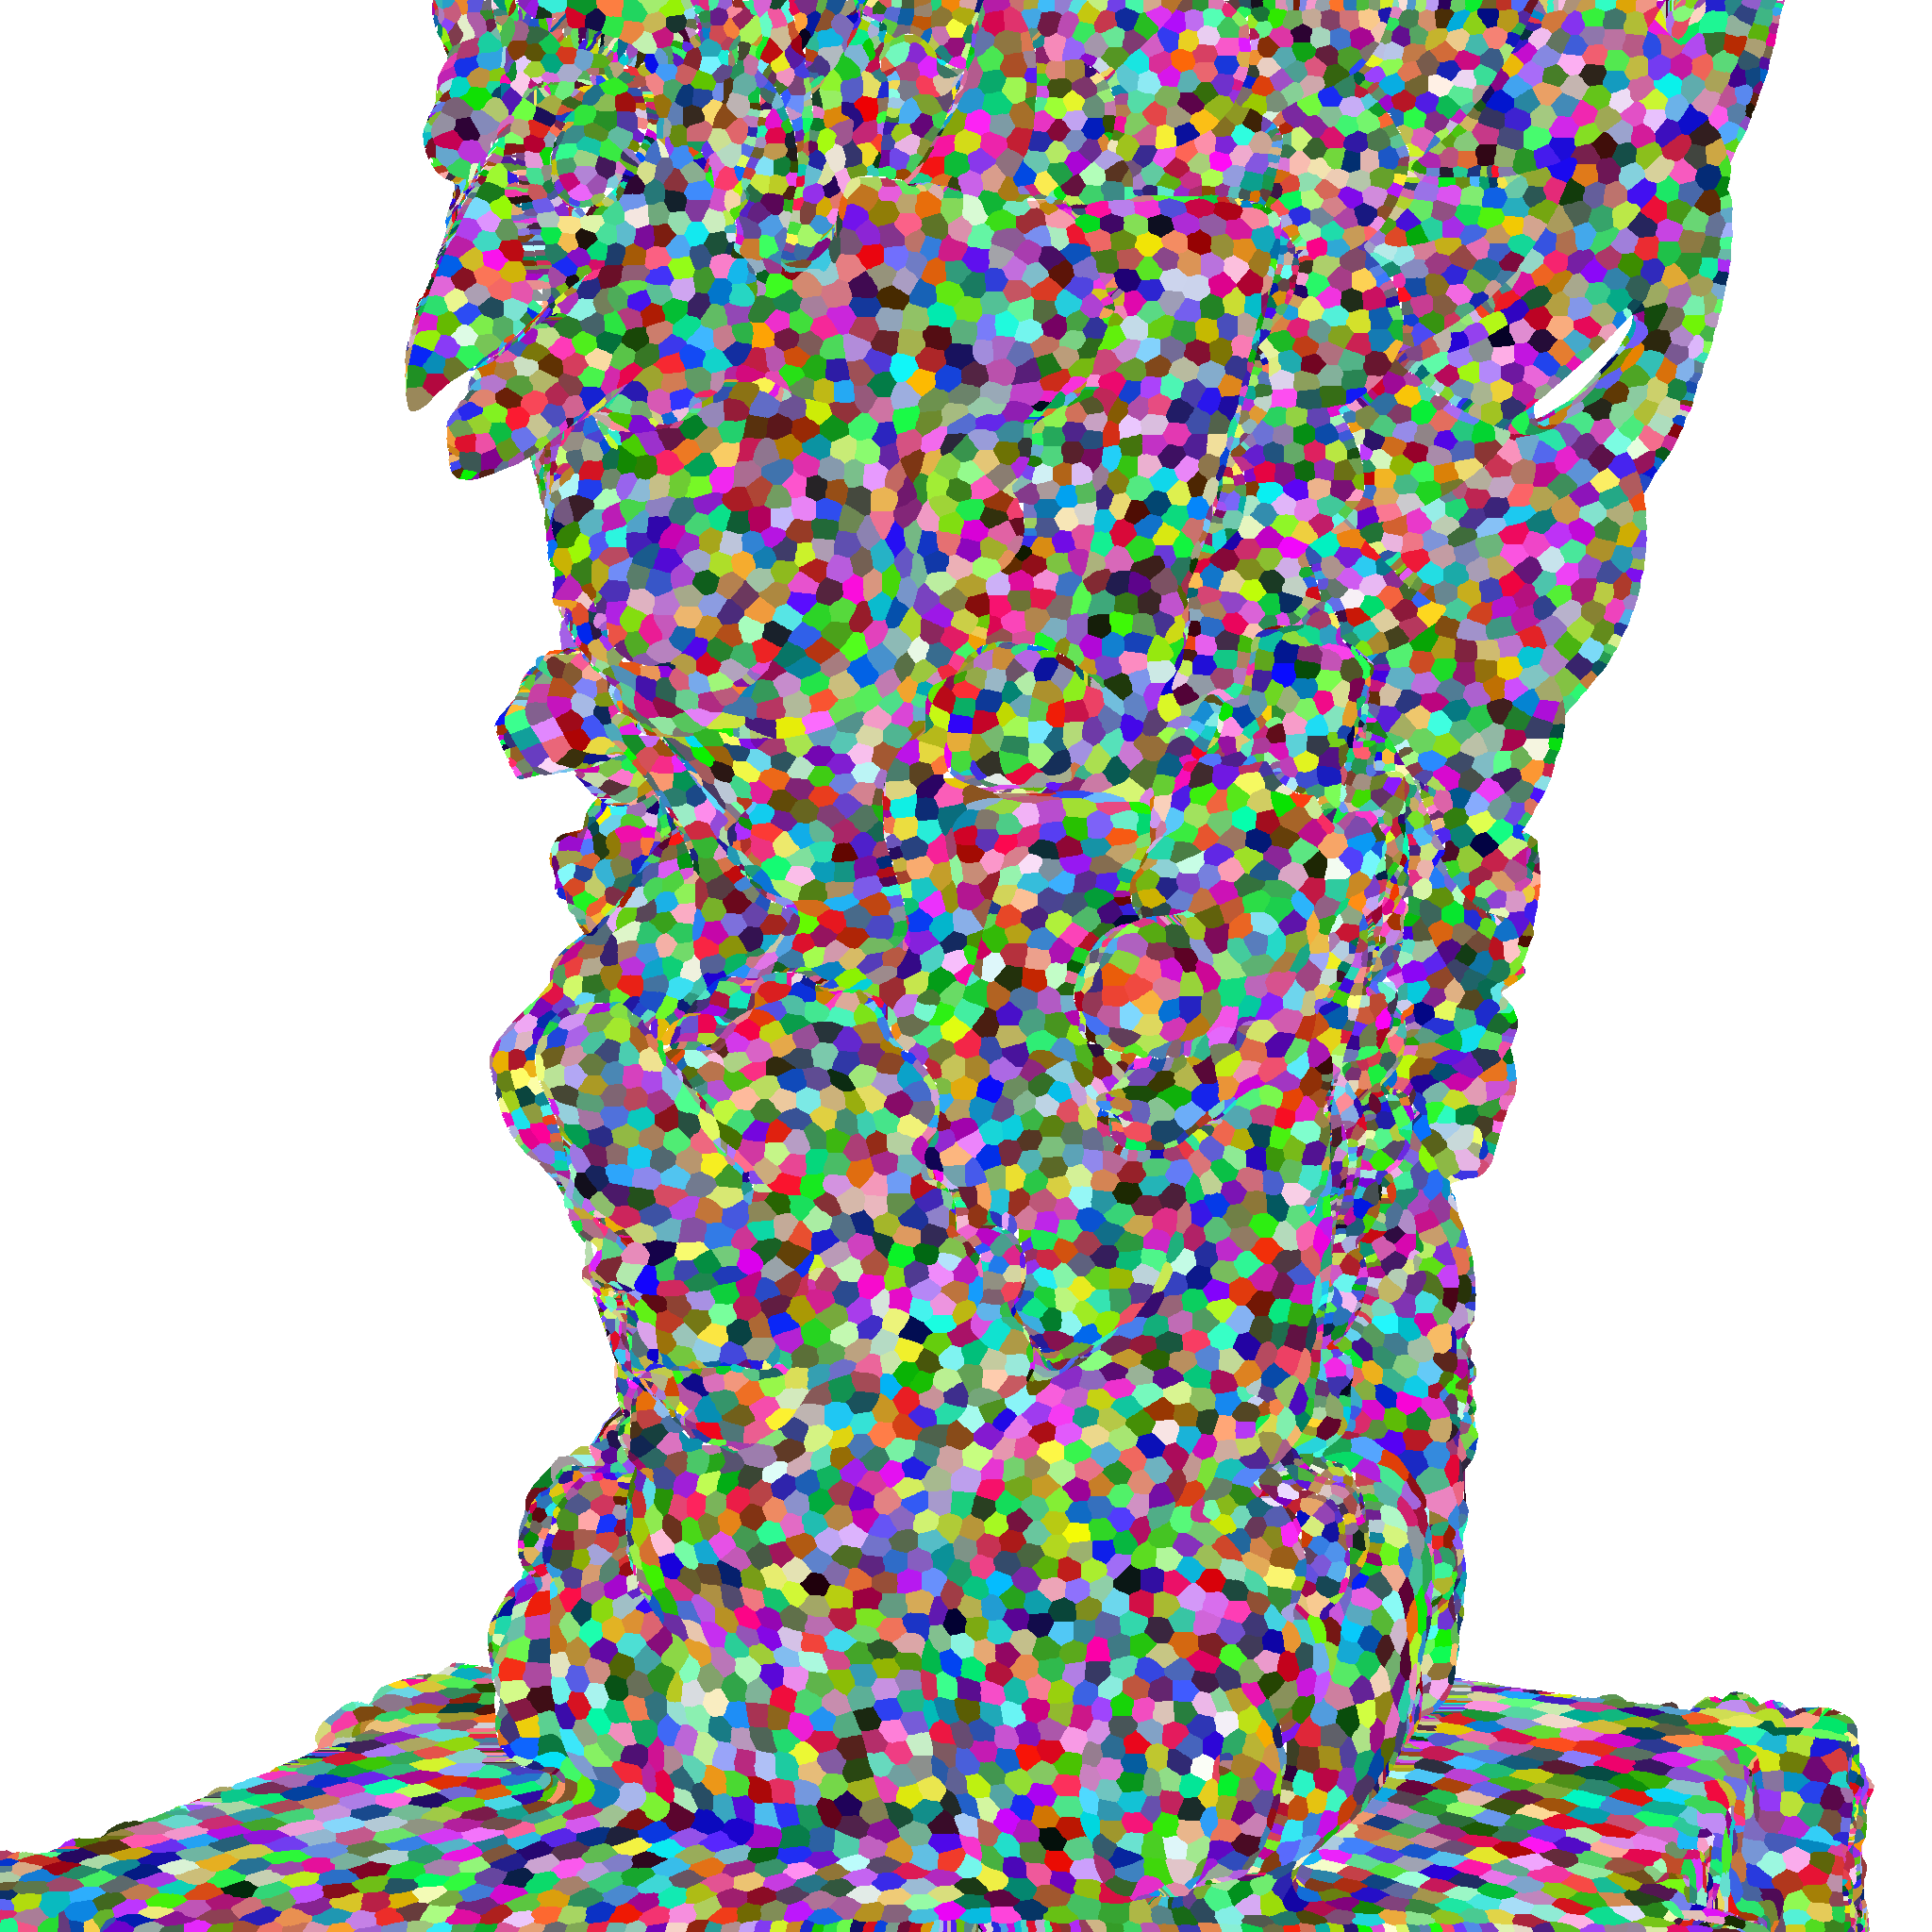
\includegraphics[scale=0.05]{VoronoiDiagram2D-Garuda}
\centering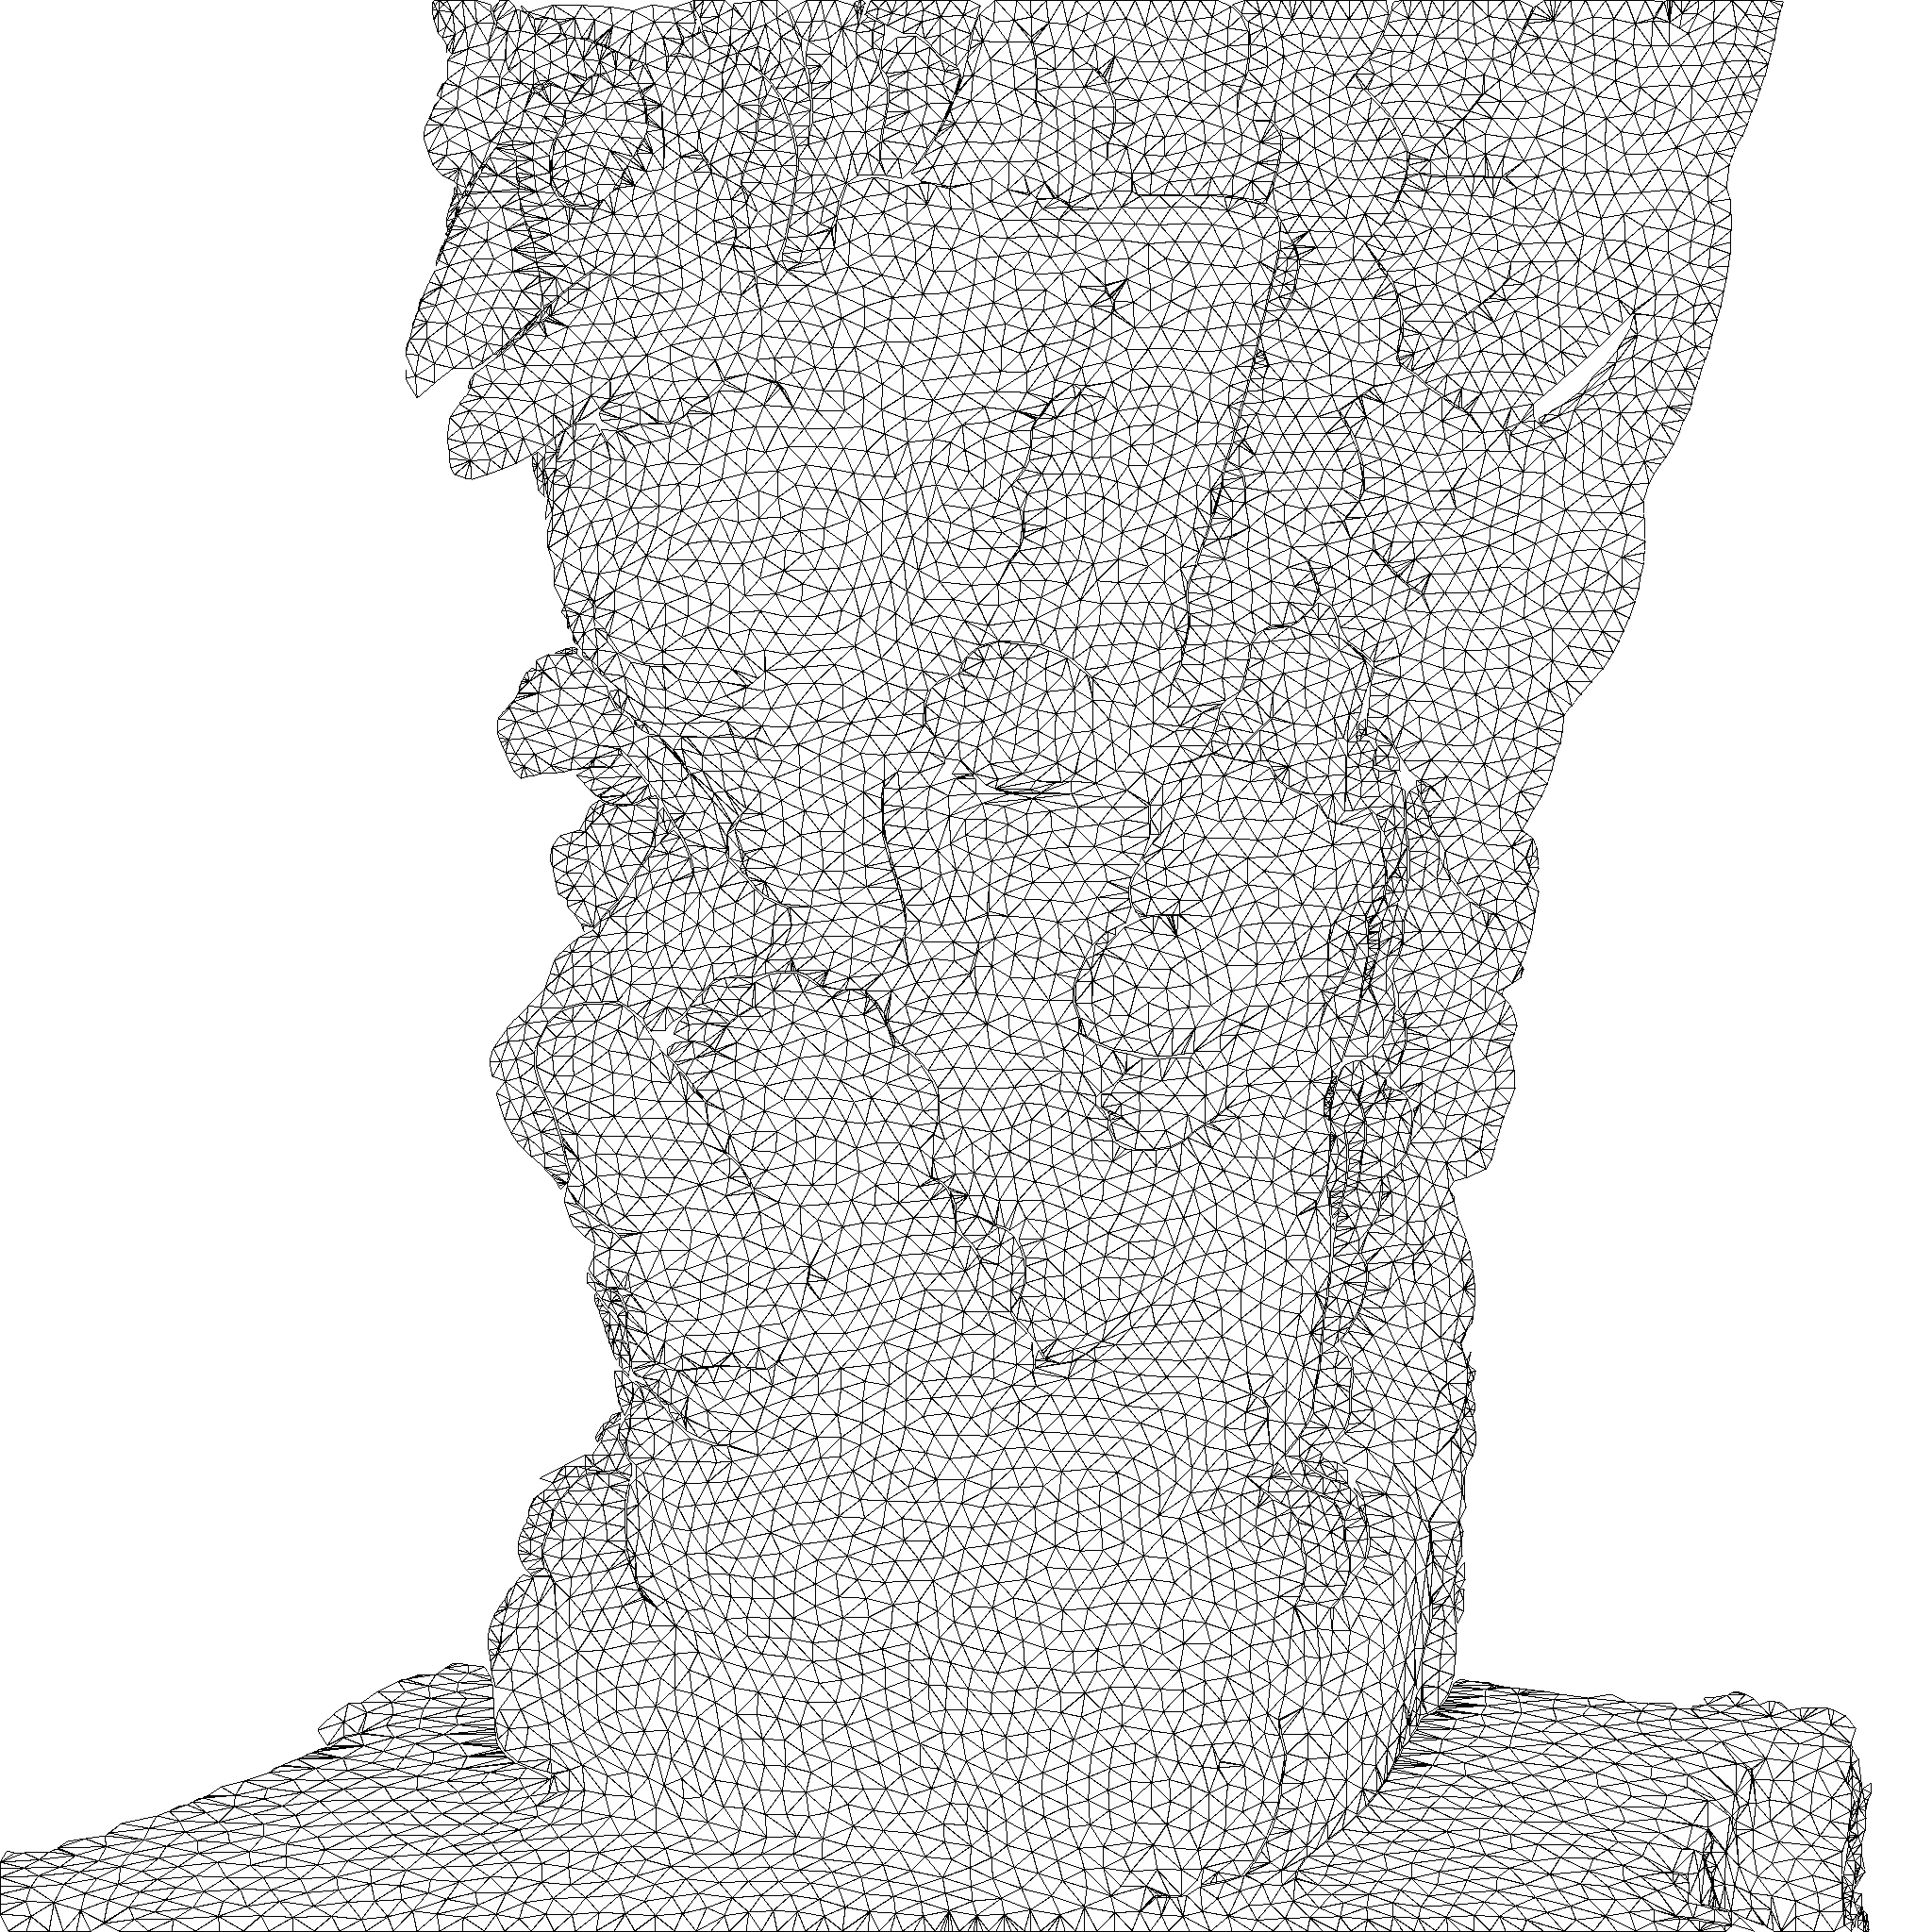
\includegraphics[scale=0.05]{Triangulation2D-Garuda}
\centering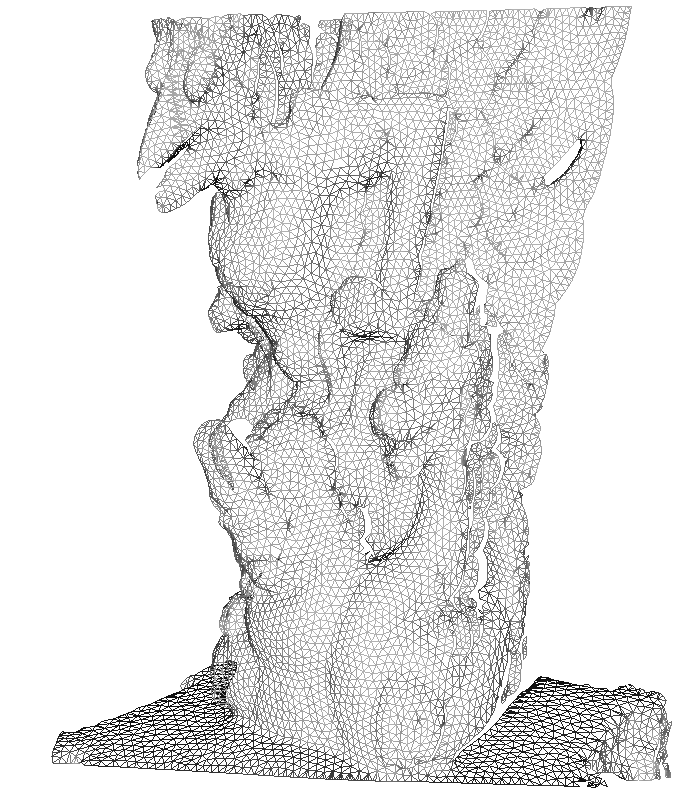
\includegraphics[scale=0.13]{Triangulation2DEmbedded-Garuda}
\caption{Voronoi diagram (a) and triangulation obtained as an altered dual representation of the Voronoi diagram (b).}
\label{fig:voronoi_diagram_triangulation}
\end{figure}

\arnaud{Add a close-up view of triangulation considering borders}

\arnaud{ADD ILLUSTRATION TRIANGULATION WITH/WITHOUT CONSIDERING BORDERS}

In order to avoid creating triangles with a bad aspect ratio (Figure ...) next to the borders of detected (due to the position of Voronoi cells sites, being the projection of the centroid on the detected border of the cell), we need to add extra sites to the Voronoi diagram, close to those regions to give triangles in this area a better aspect ratio.

For this we decide to add a site on the barycenter of each triangle whose minimum angle is below a certain threshold $\alpha$. 
This parameter will ensure that all the triangles of the mesh have no angles below this value $\alpha$.

\begin{figure}[ht]
\centering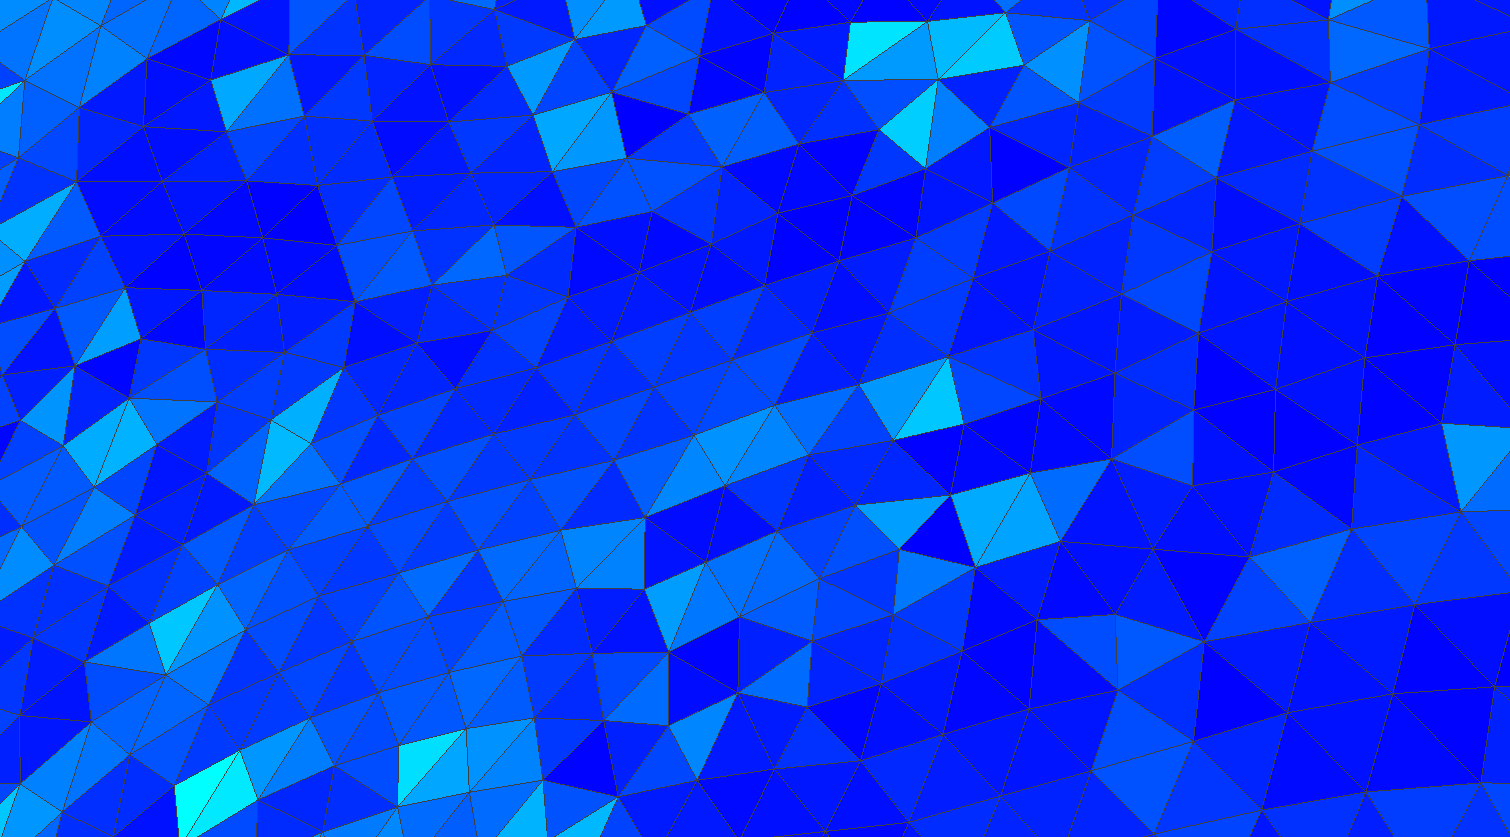
\includegraphics[scale=0.1]{Triangles-WellShaped-TechShop}
\centering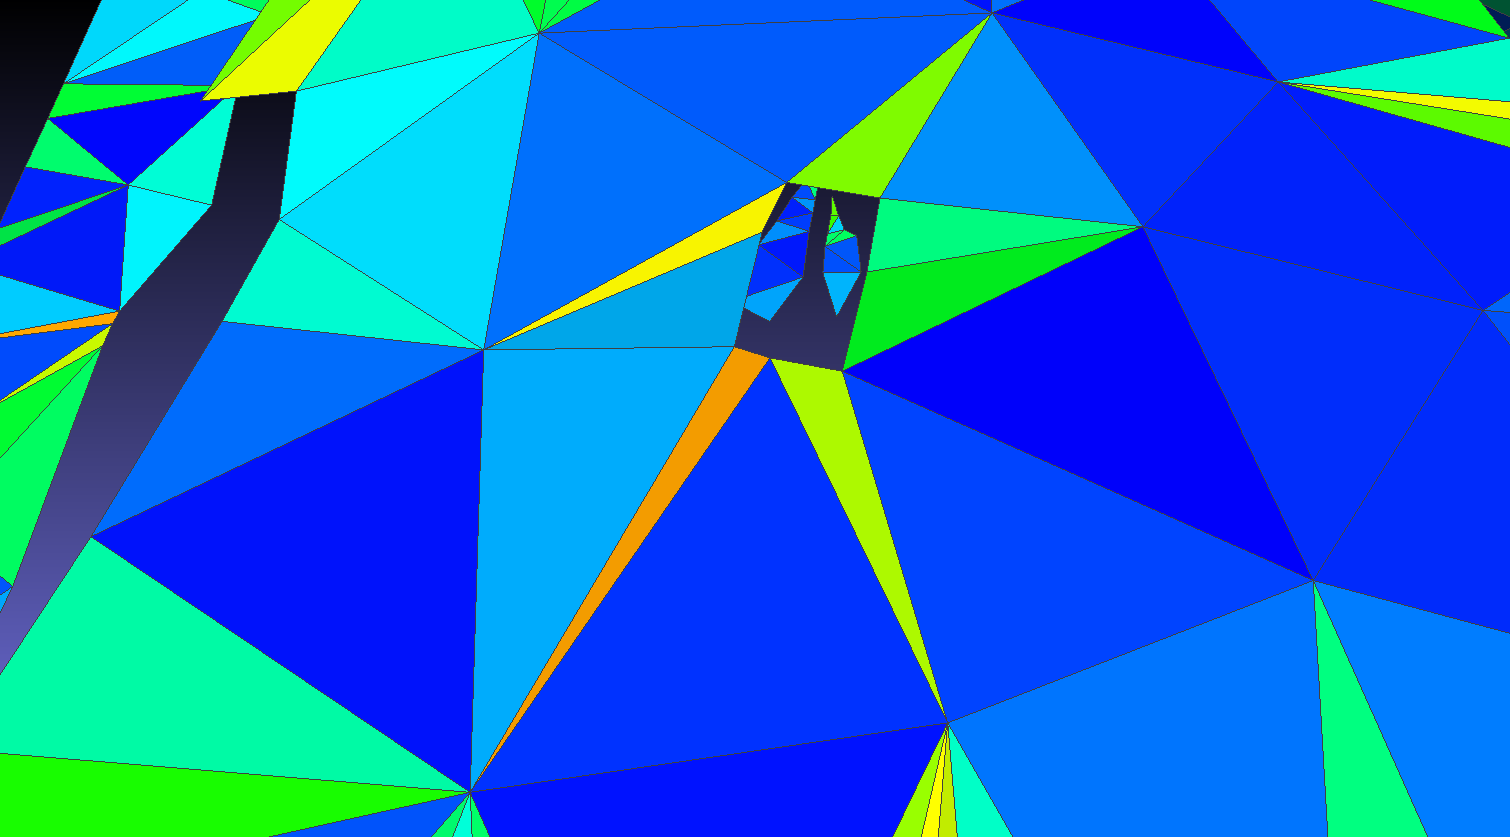
\includegraphics[scale=0.1]{Triangles-NotWellShaped-TechShop}
\caption{Parts of the triangulation of the TechShop with more (right image) or less (left image) well-shaped triangles. 
Colors vary from blue to red, from equilateral to skinny triangles.}
\label{fig:voronoi_diagram_triangulation}
\end{figure}

\subsection{Surface subdivision}

Now, to refine our base mesh, and obtain a progressive representation of the acquired data, we subdivide every triangles recursively, until reaching the same density as the original point cloud.
To do so, we divide every edge into two edges, linking both by introducing a new vertex. The position of this vertex will depend on the subdivision filter applied \cite{PR08}.
Here we will show an application considering an altered \textit{Mid-Edge subdivision} scheme.
For the subdivision we consider two different cases :
\begin{itemize}
	\item If the currenly subdivided edge is composed of two border vertices (pixels that have been marked as belonging to the border) and that this edge is on the border of the current triangulation level (Figure ...a), then the newly inserted vertex is moved to the middle of the border (Figure ...b)
	\item Otherwise, the classical Mid-Edge subdivision scheme is applied.
\end{itemize}

The subdivision process is done in the 2D domain, this means that newly inserted vertices are given a position in 2D, and their 3D position is recovered by embedding the pixel on which the new vertex is lying on.
By doing so, we always project newly inserted vertices onto original ones (the ones that have been acquired), which are on the surface acquired.

\arnaud{ADD ILLUSTRATION SUBDIVISION ON A BORDER}